\section{Well-posedness of the problem}\label{wen-sect-saw}
\subsection{Self-adjointness $\Delta$}
We are going to use the tools of functional analysis to prove that the Cauchy problem~\cref{wen-maineq} is well-posed for certain types of initial data.
We define the Hilbert space 
\begin{equation*}
\mathcal{H} = L^{2}(M,E)\oplus L^{2}(\partial M, \mathcal{P}_+ E)
\end{equation*}
with inner product\footnote{
For simplicity,
we denote $W^{n,m}(M,E)$ (resp. $W^{n,m}(\partial M, \mathcal{P}_+E)$) by $W^{n,m}(M)$ (resp. $W^{n,m}(\partial M)$)}
\begin{equation}\label{wen-innerpdt}
\langle \cdot, \cdot \rangle _\mathcal{H} = \langle \cdot, \cdot \rangle _{L^2(M)} + c \langle \cdot, \cdot \rangle _{L^2(\partial M)}
\end{equation}
One should notice that only a subspace of $E$ is considered for $\partial M$.
This is used to ensure that we have a Hilbert space for the following discussions.
We will show that $\Delta$ is self-adjoint with domain\begin{equation*}
\mathcal{D} \equiv \{ \Phi = (\phi, \phi_|) \in W^{1,2}(M)\times W^{1,2}(
\partial M)\enskip | \enskip \mathcal{P}_+\phi \vert_{\partial M} - \phi_| = 0 \}
\end{equation*}
Let us find the domain of $\Delta^*$.  
Let $\Phi = (\phi, \phi_|) \in \dom(\Delta^*)$.
Then, for any $ \Psi = (\psi, \psi_|)\in\mathcal{D}$
\begin{equation}\label{wentzell-proof-sa}
\begin{split}
\langle \Delta^*\Phi, \Psi \rangle_\mathcal{H} =
\langle \Phi, \Delta \Psi \rangle _\mathcal{H}
 = & \int_M \phi^\dagger i \gamma^0 \gamma^j \partial_j \psi 
+ \int_{\partial M} \phi^\dagger_|(  -\gamma^0\mathcal{P}_- \psi\vert_{\partial M} + ic \gamma^0 \gamma^a \partial_a\psi_|)   \\
 = & - \int_M \partial_j \phi^\dagger i \gamma^0 \gamma^j \psi 
+ \int_{\partial M} \phi^\dagger_|(-\gamma^0 \mathcal{P}_- \psi\vert_{\partial M} + ic \gamma^0 \gamma^a \partial_a  \psi_|) 
- i\phi\vert_{\partial M}^\dagger \gamma^0 \gamma^\bot \psi\vert_{\partial M}   \\
= &
- \int_M \partial_j \phi^\dagger i \gamma^0 \gamma^j \psi 
+ \int_{\partial M} - \phi^\dagger\vert_{\partial M}\mathcal{P}_- \gamma^0 \psi_| + ic \phi^\dagger_|\gamma^0 \gamma^a \partial_a  \psi_|  \\
& - i \phi\vert_{\partial M}^\dagger \gamma^0 \gamma^\bot \psi\vert_{\partial M} 
-\phi_|^\dagger \gamma^0 \mathcal{P}_- \psi\vert_{\partial M} 
+ \phi^\dagger\vert_{\partial M}\mathcal{P}_- \gamma^0 \psi_| \\
%--------------
%\underset{(\mathcal{P}_-)^\dagger = \mathcal{P}_-}{=} 
%& \langle \Delta\Phi, \Psi \rangle_\mathcal{H}
%+\phi^\dagger\vert_{\partial M} \gamma^0 (-i \gamma^\bot %\psi\vert_{\partial M} + \psi_|)
%- \phi_|^\dagger \gamma^0 \mathcal{P}_- \psi\vert_{\partial M} \\
%= & \langle \Delta\Phi, \Psi \rangle_\mathcal{H}
%------------------------
= &
- \int_M \partial_j \phi^\dagger i \gamma^0 \gamma^j \psi 
+ \int_{\partial M} - \phi^\dagger\vert_{\partial M}\mathcal{P}_- \gamma^0 \psi_| + ic \phi^\dagger_|\gamma^0 \gamma^a \partial_a  \psi_| \\
& + (\phi^\dagger\vert_{\partial M} - \phi_|^\dagger)\mathcal{P}_+ \gamma^0 \psi\vert_{\partial M}
\end{split}
\end{equation}
In the above calculation, we have implicitly assumed that $(\phi, \phi_|)\in W^{1,2}(M)\times W^{1,2}(\partial M)$.
$\Delta$ is symmetric because~\cref{wentzell-proof-sa} equals $\langle \Delta\Phi, \Psi\rangle_\mathcal{H}$ if $\Phi$ is furthermore an element of $\dom(\Delta)$.
In particular, the last line of~\cref{wentzell-proof-sa} can be rearranged as $\langle\Omega,\Phi\rangle_\mathcal{H}$ for some $\Omega\in\mathcal{H}$ if and only if the last term of~\cref{wentzell-proof-sa} disappears, \ie
$\mathcal{P}_+\phi\vert_{\partial M} - \phi_| = 0$.
Hence, the domain of $\Delta^*$ is contained in $\mathcal{D}$, which implies the self-adjointness of $\Delta$.\\\\
By the self-adjointness of $\Delta$, it follows that 
\begin{proposition}\label{wen-propwellposedness}
The Cauchy problem~\cref{wen-maineq} with initial data $\Phi_0\in\mathcal{D}$ has a unique solution $\Phi(t) = e^{-i\Delta t}\Phi_0 $
\end{proposition}
%-----------------
The self-adjointness being proven, 
we can find a generalized orthonormal basis of $\mathcal{H}$ consisting of eigenfunctions of $\Delta$.
As examples, the cases for $M = \mathbb{R}^{d-1}\times\mathbb{R}_+$ and $M = \mathbb{R}^{d-1}\times [-L, L]$ have been treated in~\cref{wen-subsect1} and~\cref{wen-subsect-saw2}.
%%%%%%%%
\begin{remark}
The assumption $c>0$ ensures the positivity of $\|\cdot\|_\mathcal{H}$. 
In the classic level, it seems that negative $c$ will lead to some physical difficulties. 
In our configuration, we allow the boundary to carry energy.
The example of~\cref{appendix-wen-shockwave} shows that we might have boundary fields whoose energies increase infinitely.
\end{remark}
%%%%%%%%
\subsection{Causal propagation}\label{wen-subsect-causal}
As a complement for~\cref{wen-propwellposedness},
we would like to show that on certain manifolds $\mathcal{M}$, 
the solution of~\cref{wen-maineq} propagates causally, \ie depending smoothly and causally on the initial data.
More explicitly, 
we would like to prove the following proposition.
\begin{proposition}\label{wen-prop-causal}
Suppose that 0 is an isolated point of the spectrum of $\Delta$. 
Let $\Sigma_0$ and $\Sigma_1$ be two equal-time surfaces.
Let $\Phi_0 = (\phi_0, \phi_{|0})\in W^{\infty,2}(M)\times W^{\infty,2}(\partial M)$ be the initial data of the problem~\cref{wen-maineq} such that
\begin{equation}\label{wen-domaindeltak}
\begin{split}
& \mathcal{P}_-\big( \partial_\bot^{2k-1}\phi\vert_{\partial M} - c^{-1}\partial_\bot^{2k-2}\phi\vert_{\partial M}\big) = 0  \\
& \mathcal{P}_+\big( \partial_\bot^{2k}\phi\vert_{\partial M} - c^{-1}\partial_\bot^{2k-1}\phi\vert_{\partial M}\big) =0  
\end{split}
\end{equation}
for all $k\in\mathbb{N}$.
Then, the solution $\Phi$ of the problem depends smoothly and causally on the initial data $\Phi_0$ in the sense that for any $\mathcal{S}_0 \subset \Sigma_0$
\begin{equation}\label{wen-causaldependence}
\big\| \frac{\partial^k}{\partial t^k} \Phi\big\|_{\mathcal{H}(\mathcal{S}_1)}
\leq
\big\| \Phi\big\|_{\mathcal{H}^{k}(\mathcal{S}_0)}
\end{equation}
for any $k\in\mathbb{N}$ and $\mathcal{S}_1 \in D^+(\mathcal{S}_0)\cap\Sigma_1$, where $D^+(\mathcal{S}_0)$ is the future domain of dependence of $\mathcal{S}_0$.
Here, the \rhs of the inequality represents the norm of the restriction of $\frac{\partial^k}{\partial t^k} \Phi$ on $\mathcal{S}_1$ and the \lhs is defined by $\|\Delta^k \Phi\|_{\mathcal{H}(\mathcal{S}_0)}$  
\end{proposition}
Let us take a pause and analyse the elements of~\cref{wen-prop-causal} in a more detailed way.
The relation~\cref{wen-causaldependence} that we try to prove states that we can control the time derivative of any order the data by the data in the causal past.
The condition~\cref{wen-domaindeltak} actually demands $\Phi$ to be in $\cap_{k\in\mathcal{N}^*}\dom(\Delta^k)$\footnote{
This can be easily proven by mathematical induction.
}.
This requirement allows us to make sense of the map
from $\mathcal{H}^k(M) = \cap_{s=1}^{k} \dom(\Delta^s)$ to $\mathbb{R}_+$
\begin{equation}\label{wen-hilbertnorm}
\| \cdot \|_{\mathcal{H}^k(M)} = \| \Delta^k \cdot \|_{\mathcal{H}(M)}
\end{equation}
In general, this map does not define a norm on $\mathcal{H}^k(M)$ because of the 0-modes of $\dom(\Delta)$ ($\ker \Delta \neq \{0\}$).
However, 
if 0 is an isolated point of the spectrum of $\Delta$, $\Delta^k \Phi$ does not vanish for all $k\in\mathbb{N}$.
In effect, 
if $\Delta^k \Phi = 0$ for a certain $k>0$,
then $\Delta^{k-1}\Phi\in\ker\Delta$, which is forbidden because $0$ is not in the spectrum of $\Delta$.
Therefore, under these assumptions, 
\cref{wen-hilbertnorm} does define a norm.
%
Consider an element $\Phi \in \mathcal{K}$.
As the time evolution of the system is given by
\begin{equation*}
i \frac{\partial }{\partial t} \Phi = \Delta \Phi 
\end{equation*}
taking into account the fact that $\Phi\in\dom(\Delta^2)$, one gets
\begin{equation}\label{wen-tobebounded}
\begin{split}
\big\| \frac{\partial }{\partial t} \Phi \big\|^2_\mathcal{H} = \| \Delta \Phi \|^2_{\mathcal{H}}  = &
\langle \Phi, \Delta^2 \Phi \rangle_{\mathcal{H}}   \\ 
\underset{\textrm{Green's formula}}=
& - \int_M \partial^j \phi^\dagger \partial_j \phi 
 -  \int_{\partial M}\phi_|^\dagger \mathcal{P}_+(\partial_\bot \phi)\vert_{\partial M} 
 + \int_{\partial M} (\phi^\dagger \partial_\bot\phi)\vert_{\partial M}
- c\int_{\partial M} \partial^a \phi^\dagger_| \partial_a \phi_| \\
\underset{\Phi \in \dom(\Delta^2)}{=} &
\|\nabla \phi \|^2_{L^2 (M)} + c^{-1} \| \mathcal{P}_- \phi\vert_{\partial M} \|^2_{L^2(\partial M)}
+ c \| \mathcal{P}_+ \nabla \phi\vert_{\partial M} \|^2_{L^2(\partial M)}
\end{split}
\end{equation}
where $\nabla$ is the gradient.
We will prove the following proposition as in~\cite{Zahn2016}
\begin{proposition}\label{wen-propcau}
With the same notations as in~\cref{wen-prop-causal},
%Let $\Sigma_0$ and $\Sigma_1$ two equal-time surfaces. 
%Then, for $\Phi = (\phi, \phi_|) \in \mathcal{K}$
% any smooth solution of \cref{wen-maineq} for smooth initial data $(\phi_0, \phi_{|0}) \in C^\infty(M) \times C^\infty(\partial M)$ on a Cauchy surface $\mathcal{S}_0 \subset \Sigma_0$,
the following relation holds
\begin{equation}\label{wen-causal}
\big\| \frac{\partial}{\partial t} \Phi \big\|_{\mathcal{H}(\mathcal{S}_1)}^2
\leq 
\big\| \frac{\partial}{\partial t} \Phi \big\|_{\mathcal{H}(\mathcal{S}_0)}^2
\end{equation}
%for any $\mathcal{S}_1 \in D^+(\mathcal{S}_0)\cap\Sigma_1$, where $D^+(\mathcal{S}_0)$ is the future domain of dependence of $\mathcal{S}_0$.
\end{proposition}
\begin{proof}
As in~\cite{Zahn2016} we introduce the following quantities
\footnote{
These quantities are not tensors because the $\phi$s are spinor fields. 
In general, under a change of frame of reference
\begin{equation*}
T_{\mu'\nu'} \neq \Lambda^\mu_{\enskip \mu'}\Lambda^\nu_{\enskip \nu'}T_{\mu \nu} 
\end{equation*}
where $\Lambda$ is the element of the Lorentz group corresponding to the change of frame.
However, 
this will not affect our proof since we are not going to use tensor properties directly in the following.
}
\begin{equation*}
\begin{split}
& T_{\mu\nu} = \partial_{(\mu} \phi^\dagger \partial_{\nu)} \phi - \frac{1}{2}g_{\mu\nu} \partial_\lambda\phi^\dagger\partial^\lambda\phi  \\
& T_{|\alpha\beta} = c\Big( \partial_{(\alpha}\mathcal{P}_+\phi^\dagger_| \partial_{\beta)}\mathcal{P}_+\phi_| - 
\frac{1}{2}h_{\alpha\beta}\big( \partial_\gamma\mathcal{P}_+\phi^\dagger_| \partial^\gamma\mathcal{P}_+\phi_|
 - c^{-2}|\mathcal{P}_- \phi\vert_{\partial M}|^2 \big)\Big) 
\end{split}
\end{equation*}
As $\phi$ is a solution for the first equation of \cref{wen-maineq},
\begin{equation*}
(i\partial_0 + i\gamma^0\gamma^j\partial_j)( i\partial_0 -i\gamma^0\gamma^j\partial_j)\phi  = 
\Box \phi= 0
\end{equation*}
where $\Box = \partial^\mu\partial_\mu$ is the d'Alembertian.
On the other hand, 
\begin{equation*}
\begin{split}
&0 = (i\gamma^\mu\gamma^0\partial_\mu\phi)^\dagger
= - i\partial_j\phi^\dagger\gamma^j\gamma^0 - i\partial_0\phi^\dagger \\
\Rightarrow \quad &
\phi^\dagger(i\overleftarrow{\partial}_j\gamma^j\gamma^0 - i\overleftarrow{\partial}_0)
(i\overleftarrow{\partial}_j\gamma^j\gamma^0 + i\overleftarrow{\partial}_0)
= \phi^\dagger \overleftarrow{\Box} = 0
\end{split}
\end{equation*}
$T_{\mu\nu}$ is thus conserved on-shell. \\\\
From the expression of $\Delta^2$ (cf~\cref{wen-domaindeltak}), 
\begin{equation*}
\Box_|\mathcal{P}_+ \phi_| = c^{-1}\mathcal{P}_+\partial_\bot \phi\vert_{\partial M}
\end{equation*}
which leads to
\begin{equation*}
\begin{split}
\partial^\alpha T_{|\alpha \beta} = & 
 \mathcal{P}_+(\partial_{(\bot} \phi^\dagger\vert_{\partial M})\partial_{\beta)}\mathcal{P}_+ \phi_| + 
c^{-1}(\mathcal{P}_-\phi^\dagger\vert_{\partial M}) \partial_\beta\mathcal{P}_- \phi\vert_{\partial M}
+c^{-1}(\mathcal{P}_-\partial_\beta\phi^\dagger\vert_{\partial M}) \mathcal{P}_- \phi\vert_{\partial M} \\ 
\underset{\Phi \in \dom(\Delta^2)}{=} & 
\partial_{(\bot}\phi^\dagger\vert_{\partial M} \partial_{\beta)}\phi\vert_{\partial M} \\
= & T\vert_{\partial M,{\bot\beta}}
\end{split}
\end{equation*}
on-shell. \\\\
One can easily verify that $T_{\mu\nu}$ and $T_{| \alpha\beta}$ satisfy the dominant energy condition, \ie for a time-like vector $\xi$ \footnote{
Even though these are not tensors, their positivitiy could still be ensured by the presence of the products of conjugated quantities.
}
\begin{equation*}
\begin{split}
T_{\mu\nu} \xi^\mu \xi^\nu \geq 0 \quad \mathrm{ and }\quad
T_{\alpha\beta} \xi^\alpha \xi^\beta \geq 0 
\end{split}
\end{equation*}
Let $\xi = e_0$, which is a Killing vector field in the static case.
Then we have $\partial^\mu T_{\mu\nu}\xi^\nu = 0$.
Using Stokes' theorem, the integral of this quantity over the zone contained between $\mathcal{S}_0$ and $\mathcal{S}_1$ which is in the future domain of dependance of $\mathcal{S}_0$ (cf~\cref{integratedzone})
%
\begin{figure}[!h]
  \centering
  %\captionsetup{width=0.8\textwidth}
  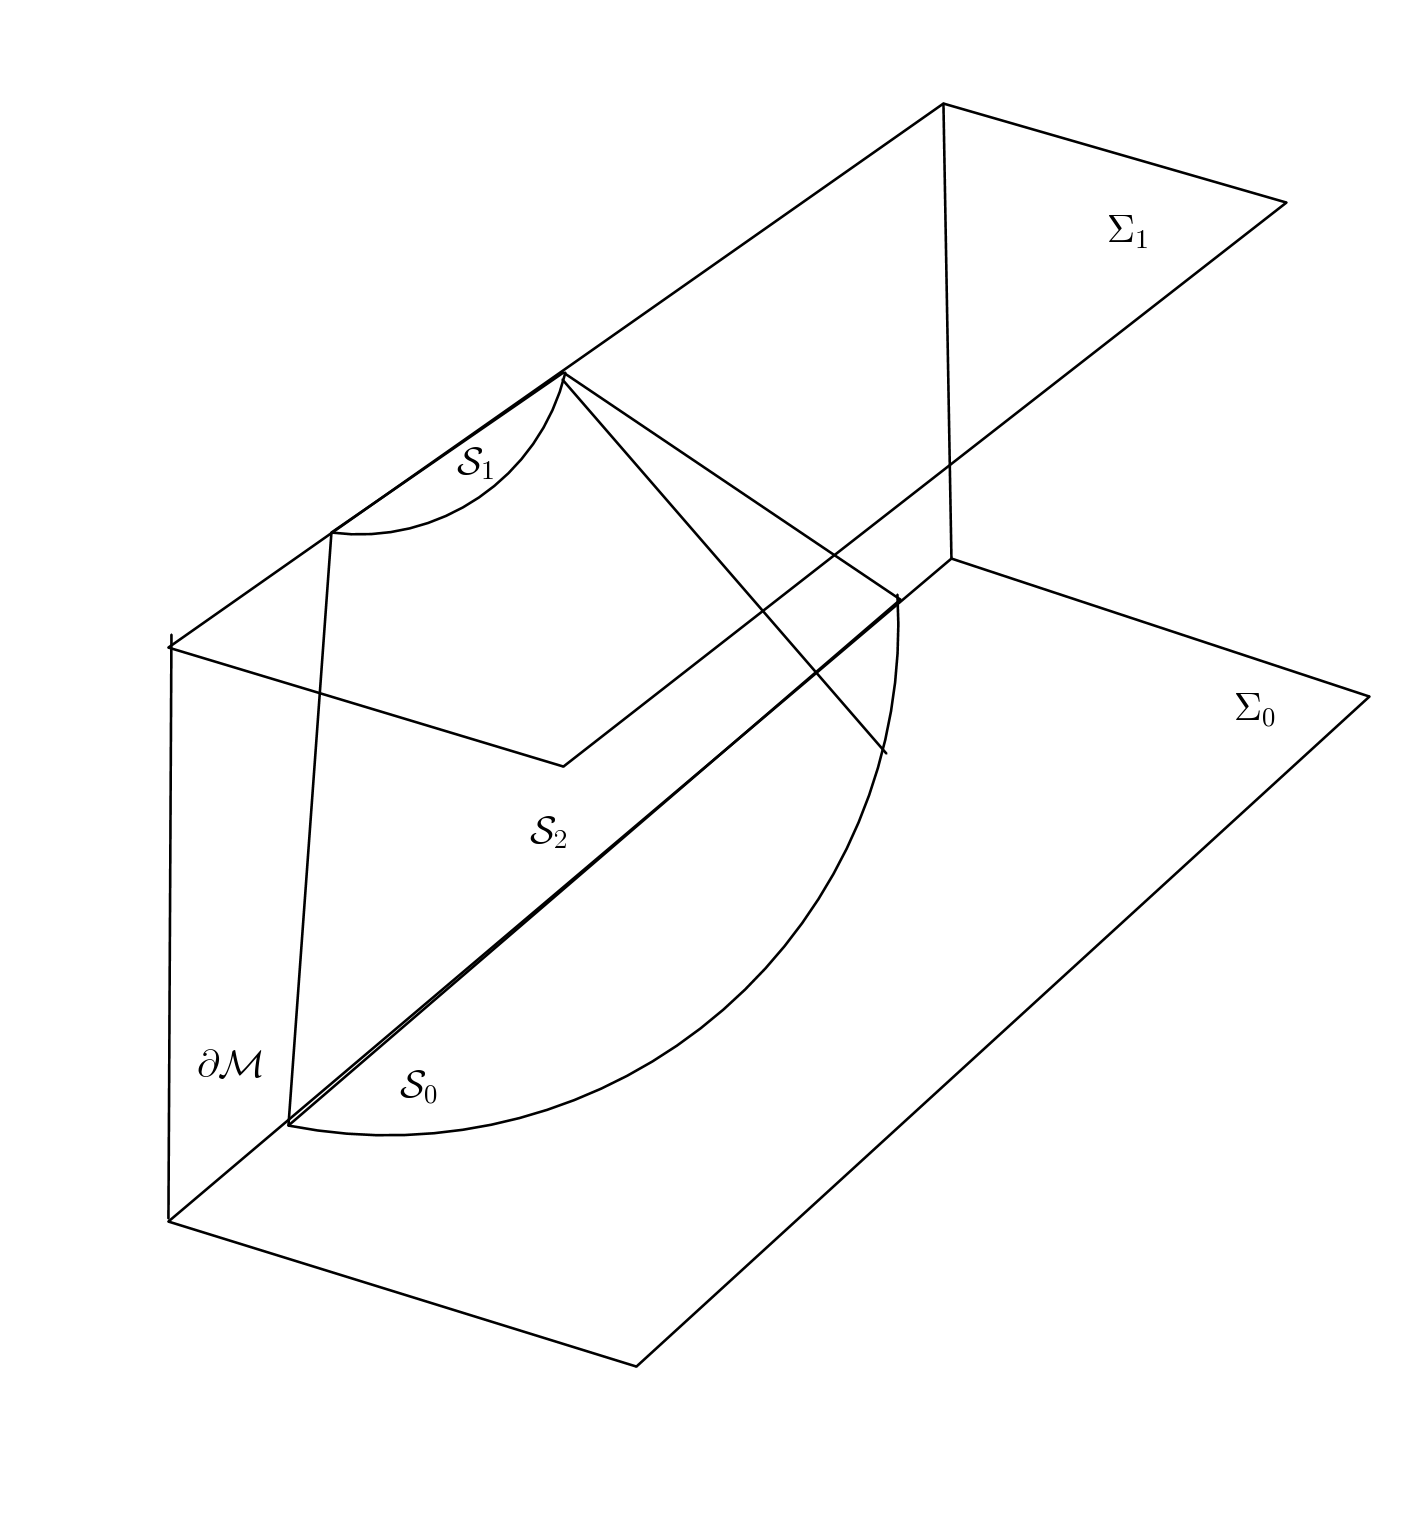
\includegraphics[height=0.4\textheight]{causal}
  \caption{Zone to integrate}\label{integratedzone}
\end{figure}
%
gives
\begin{equation*}
\begin{split}
0 \underset{\partial^\bot = -\partial_\bot}{=} &
- \int_{\mathcal{S}_0}T_{00} + \int_{\mathcal{S}_1} T_{00} + \int_{\mathcal{S}_2} n^\mu T_{\mu 0} + \int_{\partial \mathcal{M}} T \vert_{\partial \mathcal{M}, \bot 0}   \\
= & - \int_{\mathcal{S}_0} T_{00} + \int_{\mathcal{S}_1} T_{00} + 
 \int_{\mathcal{S}_2} n^\mu T_{\mu 0} -
  \int_{\partial \mathcal{M} \cap \mathcal{S}_0} T_{|00}  +\int_{\partial \mathcal{M} \cap \mathcal{S}_1} T_{|00}
 + \int_{\partial \mathcal{M} \cap \mathcal{S}_2} s^\alpha T_{\alpha 0}
\end{split}
\end{equation*}
where $n^\mu$ and $s^\alpha$ are future-directed unit vectors normal to $\mathcal{S}_2$ and $\partial M \cap \mathcal{S}_2$ respectively.
By the dominant energy condition, 
$n^\mu T_{\mu 0 }\geq 0$ and $s^\alpha T_{\alpha 0 }\geq 0$. 
We obtain \cref{wen-causal} by replacing $T_{00}$ and $T_{| 00}$ by their expression in terms of $\phi$
\end{proof}
%
To conclude, 
\cref{wen-prop-causal} is just a corollary of~\cref{wen-propcau} by using the unitary time evolution of $\Phi = e^{-i\Delta t}\Phi_0$.
\begin{remark}
As shown in~\cref{wen-subsect-saw2}, $M = [-L,L]$ is an example where 0 is an isolated point of the sepctrum of $\Delta$. 
The problem has solutions which propagate causally in this case.
\end{remark}
%%%%%%%%%%%%%%%
%%%%%%%%%%%%%%%%%%%%
%\section{Plane wave solutions in two simple cases}
%We will discuss two simple cases, $M = \mathbb{R}^{d-1} \times \mathbb{R}_+$ at first and $M = \mathbb{R}^{d-1} \times [-L, L]$ later in this section. 
%%%%%%%
%\subsection{$M = \mathbb{R}^{d-1} \times \mathbb{R}_+$}\label{wen-subsect1}
\begin{proposition}
Let $M = \mathbb{R}^{d-1} \times \mathbb{R}_+$. $\Delta$ is a self-adjoint operator with spectrum $\mathbb{R}$
\end{proposition}
\begin{proof}
The self-adjointness being proven, let us find eigenvectors and eigenvalues of $\Delta$. 
Let $k$ be an eigenvalue of $\Delta$ and $\Phi_k = (\phi_k, \phi_{| k})$. Then
\begin{equation}\label{wen-motion2}
\begin{cases}
i \gamma^0 \gamma^j \partial_j \phi_k = k \phi_k \\
-c^{-1} \gamma^0 \mathcal{P}_- \phi\vert_{\partial M} + i \gamma^0 \gamma^a \partial_a \phi_{| k} = k \phi_{| k}
\end{cases}
\end{equation}
Since for all vector $\psi$,
\begin{equation*}
(i\gamma^0 \gamma^j\partial_j - k )(i\gamma^0 \gamma^j\partial_j + k )\psi = 
(- \partial^j\partial_j - k^2) \psi = 0
\end{equation*}
has plane wave solutions, 
all vectors of the form
\begin{equation*}
\begin{split}
\phi_n = & \Big((i\gamma^0\gamma^j\partial_j + k \mathbb{1}) e^{-ip_a x^a }(A\cos p_\bot x^\bot + B \sin p_\bot x^\bot) \psi_n \\
 = &\gamma^0\gamma^a p_a (A \cos p_\bot x^\bot + B \sin p_\bot x^\bot)e^{-ip_a x^a}
+ i\gamma^0\gamma^\bot p_\bot (-A \sin p_\bot x^\bot + B \cos p_\bot x^\bot) e^{-ip_a x^a} \\
& + k \mathbb{1} e^{-ip_a x^a}(A\cos p_\bot x^\bot + B \sin p_\bot x^\bot)\Big)\psi_n  \\
\end{split}
\end{equation*}
with $p_j$ satisfying
\begin{equation*}
- p^j p_j = k^2
\end{equation*}
are solutions of the bulk equation of~\cref{wen-motion}. 
The constants $A$ and $B$ will be determined by the boundary equation of \cref{wen-motion} and the boundary condition. 
The only constraint on $\psi_n$ is that $\psi_n$ should not be in $\ker( \gamma^0 \gamma^j p_j + k \mathbb{1})$. 
\footnote{
As 
$(\gamma^0\gamma^j p_j + k \mathbb{1})
(-\gamma^0\gamma^j p_j + k \mathbb{1})  
= k^2 - (p_j)^2= 0$, 
the kernel of $\gamma^0 \gamma^j p_j + k \mathbb{1}$ is not reduced to $\{ 0 \}$
} 
Since we have projectors $\mathcal{P}_\pm$, 
it is natural to take the basis of the total representation space as the union of an orthonormal basis $\mathfrak{B}_+$ of $\ran(\mathcal{P}_+)$ and an orthonormal basis $\mathfrak{B}_-$ of $\ran(\mathcal{P}_-)$. \\\\
Considering the boundary equation of~\cref{wen-motion} and the condition that an element of $\dom(\Delta)$ should satisfy, one gets
\begin{equation}\label{wen-boundary}
\begin{split}
& \mathcal{P}_+\phi\vert_{\partial M} =  \phi_| \\
& -c^{-1} \gamma^0 \mathcal{P}_- \phi\vert_{\partial M} + i\gamma^0\gamma^a\partial_a \mathcal{P}_+\phi\vert_{\partial M} = k \phi_| 
\end{split}
\end{equation}
which implies
\begin{equation}\label{wen-boundary2}
-c^{-1} \gamma^0 \mathcal{P}_-(\phi\vert_{\partial M}) = 
\mathcal{P}_+(k\phi\vert_{\partial M} - i\gamma^0\gamma^a\partial_a\mathcal{P}_+(\phi\vert_{\partial M})) = 
i\gamma^0\mathcal{P}_-(\gamma^\bot\partial_\bot \phi\vert_{\partial M})
\end{equation}
We compute
\begin{equation*}
\begin{split}
\partial_\bot \phi \vert_{\partial M} = 
\big((\gamma^0\gamma^a p_a + k\mathbb{1})e^{-i_a x^a} p_\bot B - i\gamma^0\gamma^\bot p_\bot^2 A \big) \psi
\end{split}
\end{equation*}
Hence, \cref{wen-boundary} implies
\begin{equation}\label{wen-projected}
\mathcal{P}_- \Big( (\gamma^0 \gamma^a p_a + k\mathbb{1})(c^{-1} A - p_\bot B)
+i \gamma^0 p_\bot(c^{-1} B + p_\bot A) \Big) \psi = 0
\end{equation}
To show that the spectrum of $\Delta$ is $\mathbb{R}$, 
we construct a generalized orthonormal basis for the eigenspace consisting of eigenvectors of eigenvalue $k{\in}\mathbb{R}$.
We observe that, 
for $\psi = e_+ + e_-$ where $e_\pm \in \ran({P}_\pm)$,
\cref{wen-projected} implies
\begin{equation}\label{wen-projected2}
(\gamma^a p_a + k\mathbb{1})(c^{-1}A - p_\bot B) e_- +\gamma^0 p_\bot(c^{-1}B + p_\bot A) e_+ = 0
\end{equation}
In order to construct a generalized orthonormal basis (normalizable to the $\delta$-function),
we can take elements of $\mathfrak{B}_+ \cup \mathfrak{B}_-$ for $\psi$ in~\cref{wen-projected}.
However, as previously mentioned, we should choose $\psi$ such that $\psi\slashed{\in}\ker(\gamma^0\gamma^j p_j + k\mathbb{1})$.
As a result, there are four possible cases to be discussed: 
\paragraph{Case 1 : $\psi \in \mathfrak{B}_-$ and $p_\bot \neq 0$} 
By \cref{wen-projected2}
\begin{equation*}
(\gamma^a p_a + k\gamma^0)(c^{-1}A - p_\bot B) \psi = 0
\end{equation*}
Now, since 
\begin{equation*}
(\gamma^a p_a + k\gamma^0)^2 = ( k^2 - p^a p_a ) \mathbb{1}= p^\bot p_\bot \mathbb{1} \neq 0
\end{equation*}
we must have 
\begin{equation*}
c^{-1} A = p_\bot B
\end{equation*}
\paragraph{Case 2 : $\psi \in \mathfrak{B}_-$ and $p_\bot = 0$}
In order to have non-trivial solution, 
we must have $A \neq 0$. 
In this case, 
\cref{wen-projected2} implies 
\begin{equation*}
(\gamma^a p_a + k \mathbb{1})\psi = 0
\end{equation*}
which is not allowed because $\psi\in\ker(\gamma^0\gamma^jp_j + k\mathbb{1})$ in this case. 
This case should thus be discarded.
\paragraph{Case 3 : $\psi \in \mathfrak{B}_+$ and $p_\bot \neq 0$}
$A$ and $B$ should verify 
\begin{equation*}
c^{-1} B + p_\bot A = 0
\end{equation*}
\paragraph{Case 4 : $\psi \in \mathfrak{B}_+$ and $p_\bot = 0$}
The terms in $B$ in the expression of $\phi$ vanish because  $p_\perp = 0$ and $A$ is determined by the normalization condition.
\\\\
%The above discussion indicates that for any $k \in \mathbb{R}$, 
Therefore, for any $k\in\mathbb{R}$, 
we can find eigenvectors of $\Delta$ with eigenvalue $k$ and a corresponding generalized orthonormal basis for the eigenspace.
\end{proof}
%\subsection{${M} = \mathbb{R}^{d-1} \times [-L, L]$ }\label{wen-subsect-saw2}
The subtlety that one should beware of in this case is the projectors $\mathcal{P}_+$.
Since $\mathcal{P}_+$ is defined by considering a set of generators of Clifford Algebra on the tangent bundle $T_{ \partial \mathcal{M}}$, 
if we would like to fixe the coordinate system once for all,
we should also take into account the transformation of these generators. \\\\
Let $(x^0, \ldots, x^d)$ be the natural coordinate system of the bulk $\mathcal{M} =\mathbb{R}\times M $. 
Because of the geometric configuration of the bulk, 
this coordinate system is global. 
The boundary is therefore $\partial \mathcal{M} = \{x^d = -L \} \cup \{ x^d = L \}$.
\\\\
We denote $\{\gamma^\mu\}_\mu$ the set of gamma matrices chosen on $\{x^d  = - L \}$. 
We will have then $\mathcal{P}_+\vert_{\{x^d = L\}} = \mathcal{P}_-\vert_{\{x^d = -L\}}$ and $\gamma^\mu\vert_{\{x^d = L\}}=\gamma^\mu\vert_{\{x^d = -L\}}$ for $\mu\in\llbracket 0, d-1 \rrbracket$.
When it is not specified, we refer to the gamma matrices and the projectors on $\{x^d = -L\}$. \\\\
%
As for the boundary component $\phi_|$ of $\Phi= (\phi, \phi_|)$,
we can rewrite it as
\begin{equation*}
\phi_| = \mathbf{1}_{\{x^d = L \}}\phi_+ + \mathbf{1}_{\{x^d = - L \}}\phi_-
\end{equation*}
where $\phi_\pm$ represent the restriction of $\phi_|$ on $\{x^d = \pm L \}$.
Now, the boundary condition becomes
\begin{equation}\label{wen-saw2bound}
\begin{split}
\begin{cases}
\mathcal{P}_+ \phi\vert_{\{x^d = -L\}} = \phi_- \\
c^{-1}\mathcal{P}_-\phi\vert_{\{x^d = -L\}} = \mathcal{P}_-(\partial_d \phi\vert_{x^d = -L}) \\
\mathcal{P}_- \phi\vert_{\{x^d = L\}} =\phi_+ \\
-c^{-1}\mathcal{P}_+\phi\vert_{\{x^d = L\}} = \mathcal{P}_+(\partial_d \phi\vert_{x^d = L}) \\
\end{cases}
\end{split}
\end{equation}
As \cref{wen-subsect1}, the general solution $\phi$ in the bulk can be written as
\begin{equation*}
\phi 
 =\Big( (k \mathbb{1}+ \gamma^0\gamma^a p_a )(A \cos p_d x^d + B \sin p_d x^d)e^{-ip_a x^a}
+ i\gamma^0\gamma^d p_d (-A \sin p_d x^d + B \cos p_d x^d) e^{-ip_a x^a} \Big) \psi
 \end{equation*}
 where $\psi $ is a spinor and the Einstein summation over $a = 1, \ldots, d-1$ is applied. \\
 We compute
\begin{equation*}
\begin{split}
\partial_d \phi\vert_{x^d = \pm L }
= (\gamma^0\gamma^a p_a + k\mathbb{1})(\mp p_d A \sin p_d L + p_d B \cos p_d L)
+ i\gamma^0\gamma^d p_d(-p_d A \cos p_d L \mp p_d B \sin p_d L)\psi e^{-ip_a x^a}
\end{split}
\end{equation*}
Hence, the boundary condition leads to
\begin{equation*}
\begin{split}
0 = &\mathcal{P}_-\Bigg(
(\gamma^0\gamma^a p_a + k\mathbb{1})\Big((p_d A + c^{-1}B) \sin p_d L + (p_d B - c^{-1}A) \cos p_d L\Big) \\
& + i\gamma^0\gamma^d p_d \Big((-p_d A -c^{-1} B) \cos p_d L + (p_d B - c^{-1} A )\sin p_d L\Big) 
\Bigg)\psi
\end{split}
\end{equation*}
\begin{equation*}
\begin{split}
0 = &\mathcal{P}_+\Bigg(
(\gamma^0\gamma^a p_a + k\mathbb{1})\Big((- p_d A + c^{-1}B) \sin p_d L + (p_d B + c^{-1}A) \cos p_d L\Big) \\
& + i\gamma^0\gamma^d p_d \Big((-p_d A + c^{-1} B )\cos p_d L - (p_d B + c^{-1} A )\sin p_d L\Big) 
\Bigg)\psi
\end{split}
\end{equation*}
Once again, there are 4 possible cases to be discussed as in \cref{wen-subsect1}
%
\paragraph{Case 1 : $\psi \in \mathfrak{B}_-$ and $p_d \neq 0$}
The same argument as in~\cref{wen-subsect1} requires
\begin{equation}\label{wen-plates1}
\begin{cases}
(p_d A + c^{-1} B) \sin p_d L + (p_d B - c^{-1} A)\cos p_d L = 0 \\
(- p_d A + c^{-1}B)\cos p_d L - (p_d B + c^{-1} A)\sin p_d L = 0
\end{cases}
\end{equation}
In order to study~\cref{wen-plates1}, we discuss the following four sub-cases according to the coefficients of $\sin$ and $\cos$.
\subparagraph{Sub-case 1: $ p_d A + c^{-1} B = 0$}
\cref{wen-plates1} becomes
\begin{equation}\label{wen-plates1-1}
\begin{cases}
(c^{-2} + p_d ^2)\cos p_d L = 0 \\
(c^{-2} - p_d^2)\sin p_d L = 2 c^{-1}p_d \cos p_d L
\end{cases}
\end{equation}
We can verify easily that supposing $ c^{-2} + p_d^2 = 0 $ will lead to paradoxal situation. 
In effect, under this assumption, the second equation of~\cref{wen-plates1-1} will lead to $e^{\pm c^{-1}L} = 0$. \\
Therefore, the only solutions for this sub-case are $p_d = \pm c^{-1}$ for $L$ satisfying $\cos c^{-1} L = 0$
%
\subparagraph{Sub-case 2: $ p_d B + c^{-1}A = 0$}
By an easy calculation, we obtain the same result as in sub-case 1
%
\subparagraph{Sub-case 3: $\cos p_d L = 0 $}
Idem as in sub-case 1.
%
\subparagraph{Sub-case 4: none of the above statements holds}
\cref{wen-plates1} leads to
\begin{equation*}
\tan p_d L = \frac{-p_d B + c^{-1} A }{p_d A + c^{-1} B} = 
\frac{-p_d A + c^{-1}B}{p_d B + c^{-1} A}
\quad\Rightarrow\quad
(p_d ^2 + c^{-2})(A^2 - B^2 )= 0
\end{equation*}
One can easily verify that $p_d =  \pm i c^{-1}$ can not satisfy the relation. 
Hence, we have $A = \pm B$ and
\begin{equation}\label{wen-tan}
\tan p_d L = \frac{\mp p_d + c^{-1}}{p_d \pm c^{-1}}
\end{equation}
Note that if $p_d$ satifies~\cref{wen-tan},
$p_d$ should be reel.
%%%%%
In effect,~\cref{wen-tan} implies
\begin{equation*}
\Im (\tan p_d L ) = \frac{\Im(c^{-1} p_d^*)}{|p_d \pm c^{-1}|^2}
\end{equation*}
As the \lhs and the \rhs have opposite sign, 
the imaginary part of $p_d$ should be 0.
%
\paragraph{Case 2 : $\psi \in \mathfrak{B}_-$ and $p_d = 0$}
This case implies $A = 0$, which is forbidden because it leads to the trivial solution.
%
\paragraph{Case 3 : $\psi \in \mathfrak{B}_+$ and $p_d \neq 0$}
The relation between $A$ and $B$ becomes
\begin{equation*}
\begin{cases}
(-p_d A - c^{-1} B)\cos p_d L + (p_d B - c^{-1}A)\sin p_d L = 0  \\
(-p_d A + c^{-1}B)\sin p_d L + (p_d B + c^{-1} A)\cos p_d L = 0 
\end{cases}
\end{equation*}
This is strictly equivalent to the case 1 of this discussion.
%
\paragraph{Case 4 : $\psi \in \mathfrak{B}_+$ and $p_d = 0$}
Leads to the trivial solution. \\\\
To conclude, we give the following proposition
\begin{proposition}
In the case where $\cos c^{-1}L \neq 0$,
the eigenvalues $k$ of $\Delta$ are of form $k^2 = q^2 + p^2_d $ where $q\in\mathbb{R}^{d-1}$ and $p_d\in \mathbb{R}$ satisfying~\cref{wen-tan} and $-p^jp_j = k^2$.
Furthermore, the elements of the family $\{(\phi_{n,q,p_d}, \phi_{|n,q,p_d})\}$, where
\begin{equation*}
\phi_k = \Big(\big(i\gamma^0\gamma^a p_a+k\mathbb{1}\big)(\cos p_d x^d + \sin p_d x^d) +
i\gamma^0\gamma^d p_d(-\sin p_d x^d + \cos p_d x^d)\Big) \psi_n e^{-ip_a x^a}
\end{equation*}
, $q=(p_1,\ldots, p_{d-1})\in\mathbb{R}^{d-1}$ and $\psi_n\in\mathfrak{B}_+\cup\mathfrak{B}_-$,
form a generalized orthongonal basis of the eigenspace for eigenvalue $k$.
\end{proposition}








